%Classe de document
\documentclass[11pt,a4paper]{scrreprt}

%%%%%%%%%%%%% Les paquetages inclus maintenant dans les style bredele: %%%%%%%%%%%%%
%Francisation
%\usepackage [latin1] {inputenc} 
%\usepackage [LGR,T1] {fontenc} % Saisie fran??ais + grec
%\usepackage [greek, frenchb] {babel}
%\usepackage[babel]{csquotes}

%R?©glages g?©n?©rauxw
%\usepackage{graphicx}
%\usepackage{textcomp} %Acc??s aux symboles Euro, etc.
%\usepackage[style=authortitle,hyperref]{biblatex}
%\usepackage{fancyhdr}
%\FrenchFootnotes
%\fancyhead[LE,RO]{\thepage}
%\fancyhead[CE]{\scshape \leftmark}

%%%%%%%%%%%%% Les paquetages divers dªsactivªs: %%%%%%%%%%%%%
%\usepackage{pxfonts}
%\usepackage{lmodern}
%\makeatletter
%\DeclareGraphicsExtensions{.pdf, .jpg, .tif, .gif}
%\AddThinSpaceBeforeFootnotes
%\fancyhead[CO]{\scshape \rightmark}
%fancyfoot[CO]{}
%\pagestyle{headings}
%\pagestyle{plain}
% En-tete
%\lhead{}        \chead{En-tte}        \rhead{}
\usepackage{tikz}
\usepackage{flupstyleutf}
\bibliography{flup}
\usepackage{harmony}
\usepackage{makeidx}
\usepackage{pdfpages}
\usepackage[colorlinks=false]{hyperref}
\usepackage{musixtex}
\setlength{\parindent}{0pt} %Supprime l'indentation en début de paragraphe
\pagestyle{fancy}
\usepackage[bitstream-charter]{mathdesign}
\usepackage{multirow}
\makeindex
\begin{document}
%--------------------------PAGE DE GARDE-------------------
%----------------------------------------------------------------------
\thispagestyle{empty}
\pagenumbering{roman}
\begin{center}
\begin{LARGE}
Académie de Woluwe-Saint-Pierre
\end{LARGE}
\end{center}

\begin{center}
\begin{LARGE}
\textbf{Cours de formation musicale}
\end{LARGE}
\end{center}

\begin{center}
\vspace{5cm}
\noindent\rule{\textwidth}{0.5mm}
\begin{huge}
\textbf{Aide-mémoire de théorie \\
\vspace{2 cm}
 Formation 3}
\end{huge}
\noindent\rule{\textwidth}{0.5mm}
\end{center}

%------------------------------------INTRODUCTION--------------------
%------------------------------------------------------------------------------
\clearpage
\thispagestyle{empty}
%\addcontentsline{toc}{chapter}{\numberline{}Remerciements}
%\chapter*{Remerciements}
\begin{vcenterpage}


\paragraph{À l'attention des parents}
\paragraph{}
Ce petit aide-mémoire reprend les différentes notions de théorie correspondant à chaque degré de formation musicale à l'académie. Chaque professeur expliquera ces notions à sa manière devant les élèves, mais les pages qui suivent permettent de retrouver rapidement les différents chapitres vus pendant l'année, de façon résumée mais néanmoins précise.


\end{vcenterpage}
%--------------------------TDM ETC------------ ------------------------
%------------------------------------------------------------------------------
\newpage
\pagenumbering{roman}
\selectlanguage{french}
\lhead{Aide-mémoire de théorie}
\rhead{Formation 3}
\fancyfoot[CO]{\thepage}%ajouter CE si a marche pas
\renewcommand{\contentsname}{Sommaire}
\tableofcontents
%\sommaire
%\listoffigures
\cleardoublepage
%--------------------------CHAPITRES------------ ----------------
%------------------------------------------------------------------------------
\clearpage
\pagenumbering{arabic}
\lhead{Aide-mémoire de théorie}
\rhead{Formation 3}
\fancyfoot[CO]{\thepage}%ajouter CE si ça marche pas
\chapter{Gammes, tonalités}
\section{Gammes}
Une gamme est une suite d'intervalle. Elle peut être transposée à partir de n'importe quelle note, pour peu que les intervalles soient respectés dans leur contenance et leur ordre d'origine. Il existe de nombreuses gammes et le nombre de notes qu'elles contiennent est assez varié.

\subsection{La gamme majeure}
C'est la gamme la plus connue. Elle est fabriqué à partir d'une suite de tons et de demi-tons dans cet ordre:
\begin{center}
\fbox{1t - 1t - $\frac 1 2$ t - 1t - 1t - 1t - $\frac 1 2$ t}
\end{center}
Voici l'exemple de Do Majeur.
\begin{center}
\includegraphics{exemples/gamme_maj.pdf}
\end{center}

Il existe beaucoup d'autres gammes. Pour respecter l'ordre des tons et demi-tons dans la gamme, il faut monter ou abaisser certaines notes, en utilisant des \fetasharp{} ou \fetaflat. Voici 2 exemples:

\subsubsection{Sol Majeur}
\begin{center}
\includegraphics{exemples/sol_maj.pdf}
\end{center}

\subsubsection{Fa Majeur}

\begin{center}
\includegraphics{exemples/fa_maj.pdf}
\end{center}

\subsection{La gamme mineure}
La gamme mineure possède plusieurs formes couramment utilisées. Toutes sont malgré tout basées sur la gamme mineure \emph{antique}, qui est la seule à correspondre à son armure.

\subsubsection{Gamme mineure antique\label{min_ant}}\index{gamme mineure antique}
\begin{center}
\includegraphics{exemples/gamme_min_ant.pdf}
\end{center}

Elle est construite sur le schéma suivant: 
\begin{center}
\fbox{1t - $\frac 1 2$ t - 1t - 1t - $\frac 1 2$ t - 1t - 1t}
\end{center}
Le 7\ieme{} degré est ici appelé \emph{sous-tonique}\index{sous-tonique} et non \emph{sensible}, vu qu'il y a 1 ton entre cette note et la tonique.

\subsubsection{Gamme mineure harmonique}\index{gamme mineure harmonique}
\begin{center}
\includegraphics{exemples/gamme_min_har.pdf}
\end{center}

Pour palier à l'absence de sensible, cette gamme présente un 7\ieme{} degré haussé, devenant ainsi une sensible. Par contre, l'intervalle VI - VII d'1 ton $\frac1 2$ (seconde augmenté) rend cette gamme mélodique. Son nom  \og harmonique \fg{} indique d'ailleurs qu'elle est utilisé pour constituer l'harmonie et les accords d'une musique.

Elle est construite sur le schéma suivant: 
\begin{center}
\fbox{1t - $\frac 1 2$ t - 1t - 1t - $\frac 1 2$ t - 1t $\frac 1 2$ - $\frac 1 2$ t}
\end{center}

\subsubsection{Gamme mineure mélodique}\index{gamme mineure mélodique}
Tout en conservant la sensible introduite dans la gamme mineure harmonique, elle rétablit l'intervalle VI - VII d'1 ton, rendant la gamme beaucoup plus adaptée à l'écriture mélodique. Cette gamme, contrairement aux autres possède une forme descendante différente de la forme ascendante (montante), et qui est similaire à la gamme antique.

Elle est construite sur le schéma suivant: 
\begin{center}
\fbox{1t - $\frac 1 2$ t - 1t - 1t - 1t - 1t  - $\frac 1 2$ t}
\end{center}
\begin{center}
\includegraphics{exemples/gamme_min_mel.pdf}
\end{center}
%D'autres gammes sont souvent associées aux gammes mineures (gamme mixte, gamme bohémienne, gamme  orientale) mais il est plus logique de les considérer comme des modes à part entière\footnote{L'aberration consistant à considérer la gamme mixte comme gamme mineure -- alors que son accord parfait est majeur -- est un exemple parmi d'autres.}.

%Les autres modes ont malgré tout gardé une certaine importance, variable selon les époques et les lieux (musique populaire, jazz, musiques du monde etc.).

\subsection{L'accord parfait}\index{accord parfait}
L'accord parfait d'une gamme est composé de la 1\iere{} (tonique), la 3\ieme{} (médiante) et la 5\ieme{} (dominante) notes d'une gamme. Jouées l'une après l'autre, ces notes forment un arpège\index{arpège}.

\section{Degrés}
Chaque note dans la gamme porte un nom, en fonction de sa place. On numérote les notes de la gamme en utilisant les chiffres romains.
\begin{itemize}
\item la première (I): tonique
\item la deuxième (II): sus-tonique
\item la troisième (III): médiante
\item la quatrième (IV): sous-dominante
\item la cinquième (V): dominante
\item la sixième(VI): sus-dominante
\item la septième (VII): sensible
\end{itemize}

En mineur antique (voir \ref{min_ant} page \pageref{min_ant}), la septième note de la gamme porte le nom de sous-tonique, étant donné qu'il y a un ton au lieu d'$\frac1 2$ entre cette dernière et la tonique. Les degrés de la gamme se notent de chiffres romains.

\section{Armures}
Les altérations présentes à l'armure se présentent toujours dans un ordre précis.
\subsubsection{Ordre des dièses}\index{ordre des dièses}
FA DO SOL RÉ LA MI SI
\subsubsection{Ordre des bémols}\index{ordre des bémols}
SI MI LA RÉ SOL DO FA
\\
\\
Cette armure permet de déterminer la tonalité majeure ou mineure présente dans une partition. À chaque armure correspondent 2 tonalités: une majeure, l'autre mineure. Par facilité, on calcule d'abord la possibilité majeure, avant de calculer la relative mineure.

\subsubsection{Tonalités en dièse}
Le dernier dièse présent à l'armure correspond à la sensible de la tonalité majeure. Il suffit donc de monter d'$\frac1 2$ ton diatonique à partir de cette note (qui est toujours un \fetasharp) pour obtenir le nom de la tonalité majeure.
\subsubsection{Tonalités en bémols}
La tonique correspond à l'avant-dernier \fetaflat. Exception: Fa Majeur, dont l'armure est si \fetaflat{} (puisqu'il n'y a pas dans ce cas d'avant-dernier \fetaflat).

On peut imaginer les différentes tonalités formant une horloge: dans le sens des aiguilles d'une montre, on ajoute un \fetasharp; dans le sens contraire, on ajoute un \fetaflat.
 %%%%%%%%%%CYCLE DES QUINTES%%%%%%%%%%%
\begin{center}
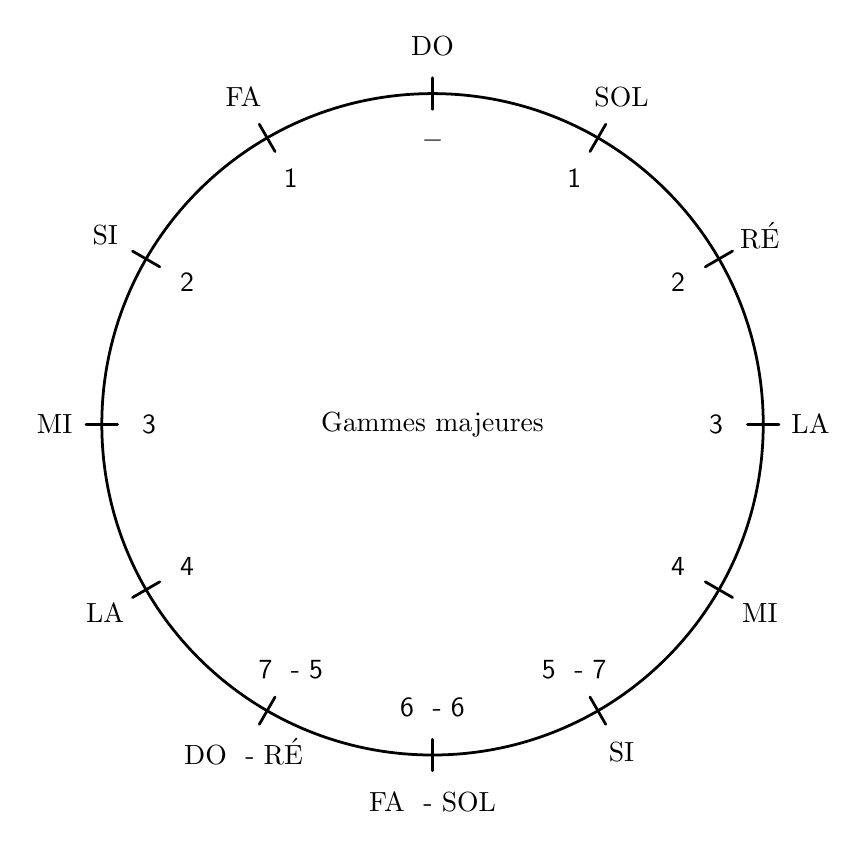
\begin{tikzpicture} [line cap=round,line width=1pt] 
\draw (0,0) circle (4.2cm);

\foreach \angle / \label in 
{0/{LA}, 30/{RÉ}, 60/{SOL}, 90/{DO}, 120/{FA}, 150/{SI \fetaflat}, 180/{MI \fetaflat},
210/{LA \fetaflat}, 240/{DO \fetasharp{} - RÉ \fetaflat}, 270/{FA \fetasharp{} - SOL \fetaflat}, 300/{SI}, 330/{MI}}
{
\draw[line width=1pt] (\angle:4.0cm) -- (\angle:4.4cm); 
\draw (\angle:4.8cm) node{\label};
}
\foreach \angle / \label in 
{0/{3 \fetasharp}, 30/{2 \fetasharp}, 60/{1 \fetasharp}, 90/{$-$}, 120/{1 \fetaflat}, 150/{2 \fetaflat}, 180/{3 \fetaflat},
210/{4 \fetaflat}, 240/{7 \fetasharp{} - 5 \fetaflat}, 270/{6 \fetasharp{} - 6 \fetaflat}, 300/{5 \fetasharp{} - 7 \fetaflat}, 330/{4 \fetasharp}}
{
\draw (\angle:3.6cm) node{\textsf{\label}};
}
\node (0,0){Gammes majeures};
\end{tikzpicture}
\end{center}

\begin{center}
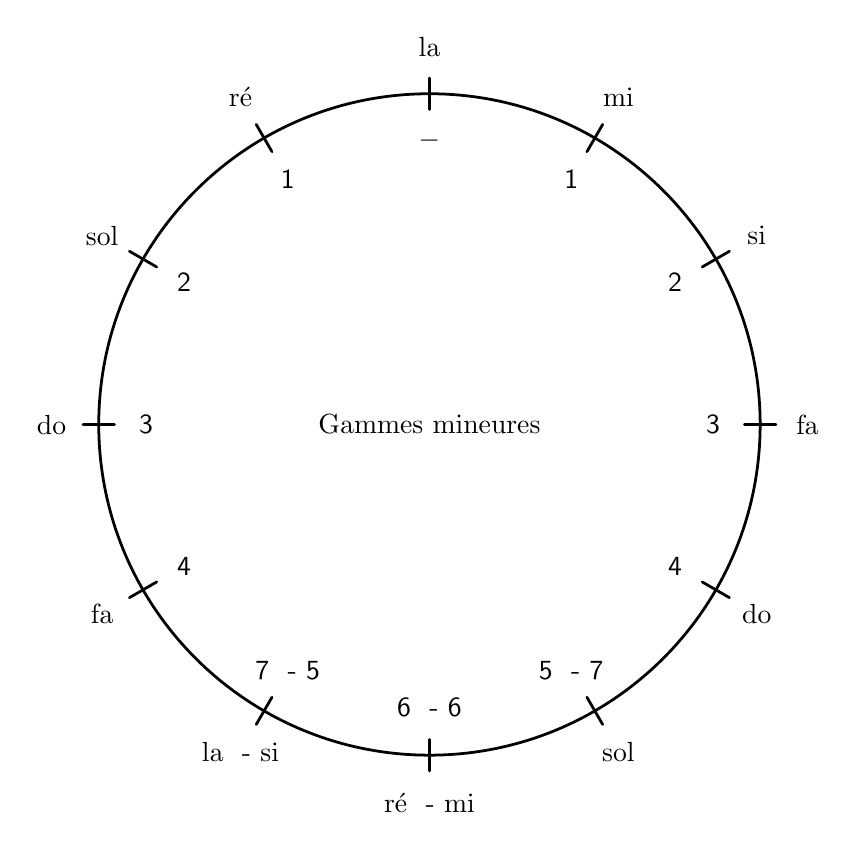
\begin{tikzpicture} [line cap=round,line width=1pt] 
\draw (0,0) circle (4.2cm);

\foreach \angle / \label in 
{0/{fa \fetasharp}, 30/{si}, 60/{mi}, 90/{la}, 120/{ré}, 150/{sol}, 180/{do},
210/{fa}, 240/{la \fetasharp{} - si \fetaflat}, 270/{ré \fetasharp{} - mi \fetaflat}, 300/{sol \fetasharp}, 330/{do \fetasharp}}
{
\draw[line width=1pt] (\angle:4.0cm) -- (\angle:4.4cm); 
\draw (\angle:4.8cm) node{\label};
}
\foreach \angle / \label in 
{0/{3 \fetasharp}, 30/{2 \fetasharp}, 60/{1 \fetasharp}, 90/{$-$}, 120/{1 \fetaflat}, 150/{2 \fetaflat}, 180/{3 \fetaflat},
210/{4 \fetaflat}, 240/{7 \fetasharp{} - 5 \fetaflat}, 270/{6 \fetasharp{} - 6 \fetaflat}, 300/{5 \fetasharp{} - 7 \fetaflat}, 330/{4 \fetasharp}}
{
\draw (\angle:3.6cm) node{\textsf{\label}};
}
\node (0,0){Gammes mineures};
\end{tikzpicture}
\end{center}


\chapter{La mesure}
\section{Les chiffres de mesure}\index{chiffres de mesure}
Les chiffres de mesure comptent toujours 2 nombres:
\begin{itemize}
\item le premier (au-dessus) indique le nombre de pulsations par mesure
\item le deuxième (en-dessous) indique la valeur de chaque pulsation
\end{itemize}

Pour savoir à quelle valeur correspond le deuxième nombre, on divise une ronde:
\begin{itemize}
\item 1 = une ronde
\item 2 = une blanche (la moitié d'une ronde)
\item 4 = une noire (le quart d'une ronde)
\item 8 = une croche (le huitième d'une ronde)
\end{itemize}
Une mesure \metric{2}{4} indique donc 2 temps par mesure, chaque temps valant une noire. Une mesure \metric{2}{2} indiquera aussi 2 temps par mesure, mais chaque temps vaudra alors une blanche.

\section{Mesures binaires et ternaires}
\subsection{Mesures binaires}\index{binaire}
Les mesures binaires sont les mesures dont les temps sont divisibles par 2: \metric{2}{4}, \metric{3}{4}, \metric{4}{4}, etc. On les appelle aussi \emph{mesures simples}.\index{mesure simple}

\subsection{Mesures ternaires}\index{ternaire}
Les mesures ternaires sont les mesures dont les temps sont divisibles par 3: \metric{6}{8}, \metric{9}{8}, \metric{12}{8}, etc. Même si \metric{6}{8} indique une mesure de 6 croches, il ne s'agit généralement pas d'une mesure à 6 temps (sauf en tempo lent), mais d'une mesure à 2 temps, chaque temps valant 3 croches (ou une noire pointée). On les appelle aussi \emph{mesures composées}.\index{mesure composée}

\section{La barre de reprise}
Pour indiquer qu'il faut répéter une ou plusieurs mesures, on utilise parfois des barres de reprises. Toutes les mesures comprise entre 2 barres de reprises (ou entre le début et une barre de reprise) doivent être rejouées. Cela permet de ne pas devoir ré-écrire un passage complet et d'économiser de la place.

\includegraphics{exemples/reprise}

\chapter{Les clés}
\fancyfoot[CO]{\thepage}%ajouter CE si ça marche pas
\section{Les clés}
Il existe 3 sortes de clés différentes: 
\begin{description}
\item [clé de sol:] (2\ieme{} ligne)\index{cle de sol@clé de sol}
\item [clés de fa:] (4\ieme{} ou 3\ieme{} ligne)\index{cle de fa@clé de fa}
\item  [clés d'ut:*] (1\iere, 2\ieme, 3\ieme{} ou 4\ieme{} ligne)\index{cle d'ut@clé d'ut}
\end{description}
Dans cet exemple, le do du milieu du piano est écrit dans les 7 clés différentes:

\centerline{\includegraphics{exemples/ex_cles.pdf}}

Chaque instrument utilise une ou plusieurs clés, en fonction de son nombre de portées et de sa tessiture. Certaines clés seront donc plutôt utilisées par les instruments graves, d'autres par les instruments aigus. Ainsi le do grave en clé de sol s'écrira do aigu en clé de fa.

\centerline{\includegraphics{exemples/do_clesol_clefa.pdf}}

Actuellement on n'utilise couramment que 4 clés: clés de sol et fa, la clé d'ut 3\ieme{} ligne (pour l'alto) et la clé d'ut 4\ieme{} ligne (pour certaines parties du violoncelle, au basson ou au trombone). Les 3 autres sont utilisées pour la transposition ou dans les partitions de musique ancienne.

\chapter{Les intervalles}\index{intervalle}
\section{Intervalles}
Un intervalle est la distance entre deux notes. Elle se calcule de plusieurs façons:
\begin{description}
\item[nom de l'intervalle:] en fonction du nombre de notes de l'intervalle (voir plus bas) 
\item[contenance:]\index{contenance} le nombre de tons et demi-tons contenus de l'intervalle
\item[qualification:]\index{qualification} la combinaison des 2 précédents, qui qualifie l'intervalle de majeur, mineur, juste, augmenté ou diminué
\end{description}

\section{Tons et demi-tons}
Le ton est constitué de l'addition d'un demi-ton diatonique et d'un demi-ton chromatique.
\subsubsection{Le demi-ton diatonique}\index{diatonique}
C'est le demi-ton situé entre deux notes de noms différents. Exemples: mi -- fa ou do \fetasharp{} -- ré. Il compte 4 commas\footnote{Le comma est une subdivision du ton. Par convention et simplification, on considère que le ton en compte~9.}.
\subsubsection{Le demi-ton chromatique}\index{chromatique}
C'est le demi-ton situé entre 2 notes de nom identique. Il compte 5 commas. Exemple: si -- si \fetaflat

\section{Calcul de l'intervalle}
%Par convention et de façon à maintenir la logique tonale, on maintient la différence écrite et logique entre ces deux demi-tons, malgré l'absence de différence sonore.

\subsection{Les noms d'intervalles}
\begin{description}
%\item [1 note:] prime
\item [2 notes:] seconde
\item [3 notes:] tierce
\item [4 notes:] quarte
\item [5 notes:] quinte
\item [6 notes:] sixte
\item [7 notes:] septième
\item [8 notes:] octave
\end{description}
Il existe évidemment des intervalles plus grands; leur nom est très facile à retenir: neuvième (9 notes), dixième (10 notes), onzième (11 notes) etc.\\

\textbf{Rappel}: on compte toujours la note de départ, celle d'arrivée et toutes celles qui sont située entre les 2.
\subsection{La contenance}\index{contenance}
Il s'agit de la quantité de tons et demi-tons contenue dans un intervalle. Attention aux additions de demi-tons!

\subsection{La qualification}\index{qualification}
Il s'agit d'un qualificatif attribué à chaque intervalle, en fonction de son nom et de sa contenance. Il n'existe qu'un seul intervalle portant le même nom et ayant la même contenance.

Certains intervalles peuvent être \emph{majeurs} (M) ou \emph{mineurs} (m). D'autres ne peuvent pas l'être mais pourront être \emph{justes}. Tous les intervalles peuvent également être augmentés et diminués.\\


En résumé:
\begin{enumerate}
\item quartes, quintes, octaves peuvent être justes, augmentées, diminuées
\item secondes, tierces, sixtes, septièmes peuvent être majeures, mineures, augmentées, diminuées.
\end{enumerate}

\subsection{Le renversement}\index{renversement}
Un intervalle peut-être renversé: on fait passer une des 2 notes par-dessus ou par-dessous l'autre, sans changer le nom des notes. La qualification d'un intervalle est inversée en cas de renversement. Exemple: en renversant une sixte mineure, on obtiendra une tierce majeure.

\centerline{\includegraphics[width=5cm]{exemples/renversement}}

\subsection{Le redoublement}\index{redoublement}
Un intervalle redoublé est un intervalle plus grand qu'une octave. Sa qualification se calcule en ne tenant compte que de l'intervalle dépassant l'octave juste. Exemple: une neuvième de 6 tons et $\frac2 2$ aura la même qualification qu'une seconde de 1 ton.\\

\pagebreak
Voici un tableau récapitulatif des contenances et qualifications d'intervalles de base.
\begin{center}
\begin{tabular}[width=15cm]{|c|c|c|c|c|c|}
\hline
Nom & diminuée & mineure & juste & majeure & augmentée\\
\hline
&&&&&\\
\multirow{2}{*} {seconde} &&\includegraphics[width= 2.35cm]{exemples/secondemin}&&\includegraphics[width= 2.35cm]{exemples/secondemaj}&\\
& & $\frac 1 2$ ton d & & 1 ton & \\ 
&&&&&\\ \hline
&&&&&\\
\multirow{2}{*} {tierce} &&\includegraphics[width= 2.35cm]{exemples/tiercemin}&&\includegraphics[width= 2.35cm]{exemples/tiercemaj}&\\
& & 1 ton $\frac1 2$ d & & 2 tons & \\
&&&&&\\ \hline
&&&&&\\
\multirow{2}{*} {quarte} && &\includegraphics[width= 2.35cm]{exemples/quartejuste}&&\includegraphics[width= 2.35cm]{exemples/quarteaug}\\
& & & 2 tons $\frac1 2$ d & & 3 tons\\
&&&&&\\ \hline
&&&&&\\
\multirow{2}{*} {quinte} &\includegraphics[width= 2.35cm]{exemples/quintedim}& &\includegraphics[width= 2.35cm]{exemples/quintejuste}&&\\
& 2 tons $\frac2 2$ d & & 3 tons $\frac1 2$ d & & \\
&&&&&\\ \hline
&&&&&\\
\multirow{2}{*} {sixte} &&\includegraphics[width= 2.35cm]{exemples/sixtemin}&&\includegraphics[width= 2.35cm]{exemples/sixtemaj}&\\
& & 3 tons $\frac2 2$ d & & 4 tons $\frac1 2$ d & \\
&&&&&\\ \hline
&&&&&\\
\multirow{2}{*} {septième} &&\includegraphics[width= 2.35cm]{exemples/septmin}&&\includegraphics[width= 2.35cm]{exemples/septmaj}&\\
& & 4 tons $\frac2 2$ d& & 5 tons $\frac12$ d & \\
&&&&&\\ \hline
&&&&&\\
\multirow{2}{*} {octave} && &\includegraphics[width= 2.35cm]{exemples/octavejuste}&&\\
&  & & 5 tons $\frac2 2$ d & & \\
&&&&&\\
\hline
\end{tabular}
\end{center}



\chapter{Termes musicaux}

Voici quelques termes musicaux ainsi que leur signification. Ces termes sont souvent en italien.

\section{Nuances}\index{nuances}
\begin{description}
\item \fetap : doux, doucement (\emph{piano} en italien)
\item \fetaf : fort (\emph{forte} en italien)
\item \fetamf : modérément fort (\emph{mezzo forte} en italien)
\item \fetamp : modérément doux (\emph{mezzo piano} en italien)
\item Crescendo\index{crescendo} (<): en augmentant l'intensité du son
\item Decrescendo\index{decrescendo} (>): en diminuant l'intensité du son
\end{description}

\section{Tempo et mesure}
\begin{description}
\item Lento: lent
\item Adagio: à l'aise
\item Andante: allant
\item Moderato: modéré
\item Allegro: rapide, joyeux
\item \metric{c}{0}: mesure \metric {4}{4}\index{\metric{c}{0}}
\item \metric{c}{1}: mesure \metric {2}{2}\index{\metric{c}{1}}
\end{description}

\section{Divers}
\begin{description}
\item Anacrouse\index{anacrouse}: mesure incomplète au début d'un morceau de musique
\item Da capo (D. C.): reprendre au début 
\item Équisonance\index{equisonance@équisonance} ou enharmonie\index{enharmonie}: note de même son, mais de nom différent. Exemples: si~--~do~\fetaflat{} ou fa~\fetasharp{} -- sol \fetaflat.
\item Staccato\index{staccato} (piqué): les notes sont jouées de façon courte. Le point est placé sous ou au-dessus de la note (à l'opposé de la hampe)
\item \includegraphics{exemples/staccato.pdf}
\item Legato\index{legato} (lié): les notes sont jouées sans interruption du son entre elles.
\item \includegraphics{exemples/legato.pdf}
\item Poco a poco: peu à peu, petit à petit
\item Tessiture\index{tessiture}: c'est l'ensemble des notes qu'un instrument peut jouer, du grave jusqu'à l'aigu. Elle permet de dire si un instrument est grave ou aigu.
\end{description}
\newpage
\addcontentsline{toc}{chapter}{\numberline{}Index}
\printindex
\end{document}